\documentclass[12pt]{article}
\usepackage{makeidx}
\usepackage{multirow}
\usepackage{multicol}
\usepackage[dvipsnames,svgnames,table]{xcolor}
\usepackage{graphicx}
\usepackage{epstopdf}
\usepackage{ulem}
\usepackage{hyperref}
\usepackage{amsmath}
\usepackage{amssymb}
\author{Omkar Mohite}
\title{}
\usepackage[paperwidth=595pt,paperheight=841pt,top=72pt,right=72pt,bottom=72pt,left=72pt]{geometry}

\makeatletter
	\newenvironment{indentation}[3]%
	{\par\setlength{\parindent}{#3}
	\setlength{\leftmargin}{#1}       \setlength{\rightmargin}{#2}%
	\advance\linewidth -\leftmargin       \advance\linewidth -\rightmargin%
	\advance\@totalleftmargin\leftmargin  \@setpar{{\@@par}}%
	\parshape 1\@totalleftmargin \linewidth\ignorespaces}{\par}%
\makeatother 

% new LaTeX commands


\begin{document}


\begin{center}
\textbf{{\LARGE Understanding the code}}
\end{center}

{\raggedright
Using Arduino we processed the data for attention level of the person. Following
is the reference site to perform the above action:
}

{\raggedright
\href{https://learn.sparkfun.com/tutorials/hackers-in-residence---hacking-mindwave-mobile}{https://learn.sparkfun.com/tutorials/hackers-in-residence---hacking-mindwave-mobile}
}
\begin{center}
	\graphicspath{ {images/} }
	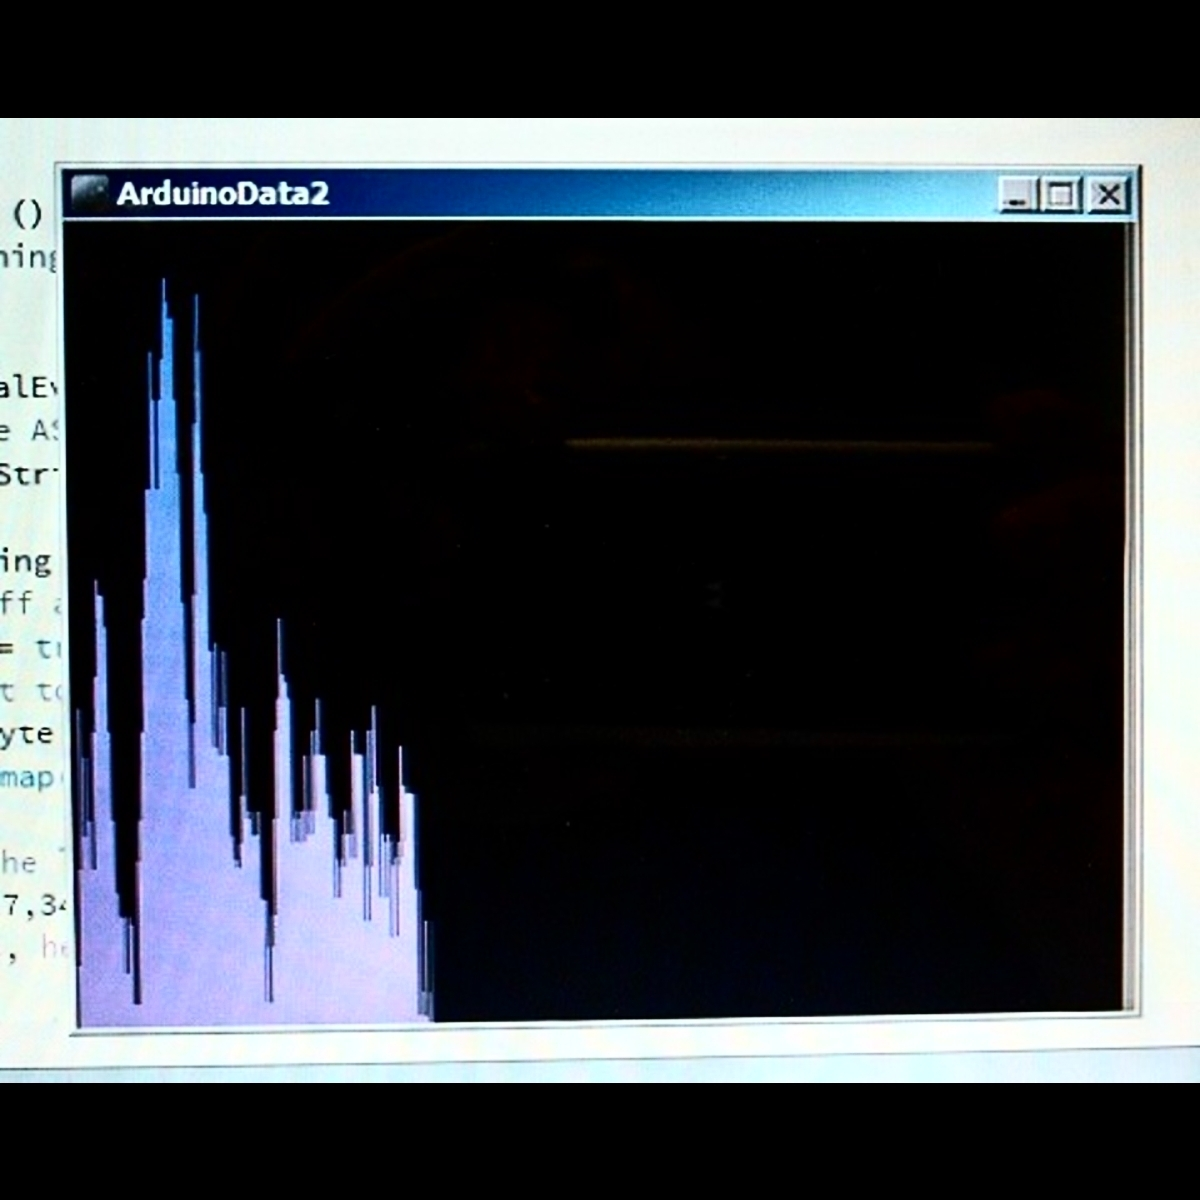
\includegraphics[width=8cm, height=8cm]{Arduino}
\end{center}
\textbf{{\large Steps:}}

\begin{itemize}
	\item Download the Processing software for Arduino.
	\item Burn the programs present in the above site for attention level detection.
	\item Wear the headset on the head.
	\item Observe the graph on your laptop/PC.
\end{itemize}

\break

{\raggedright
\textbf{{\large Program Descriptions:}}
}

\begin{enumerate}
	\item \textbf{{\large Program to  display on LCD and LED bar graph the attention level of the person}}

\begin{enumerate}
	\item \textbf{Algorithm{\large  :}}

\begin{enumerate}
\item Initialize all required ports.
\item Check for two consecutive SYNC bytes ‘AA’.
\item Check for third byte which is the payload length.
\item If payload length is 0x20, then store the next 32 bytes in an array. If payload length is 0x04 then move to step no. 11
\item Calculate the generated checksum.
\item If the last byte i.e. checksum byte of the data packet is equal to the generated checksum then check for 28th byte of the array.
\item If 28th byte is 0x04, then attention detected.
\item Then 29th byte indicates attention level of the person between 0-100.
\item If attention level lies between 0-10, it indicates mind wandering level. Indicated it with 1 LED glow.
\item If attention level lies between 10-30, it indicates poor attention level. Indicate with 2 to 3 LEDs glow.
\item If attention level lies between 40-60, it indicates neutral. Indicate it with 4-5 LEDs glow.
\item If attention level lies between 60-80, it indicates slightly elevated. Indicate with 6-7 LEDs glow.
\item If attention level is above 80, it means elevated level of attention. Indicate with all LEDs glow.
\end{enumerate}
	\end{enumerate}
\break

\begin{center}
	\graphicspath{ {images/} }
	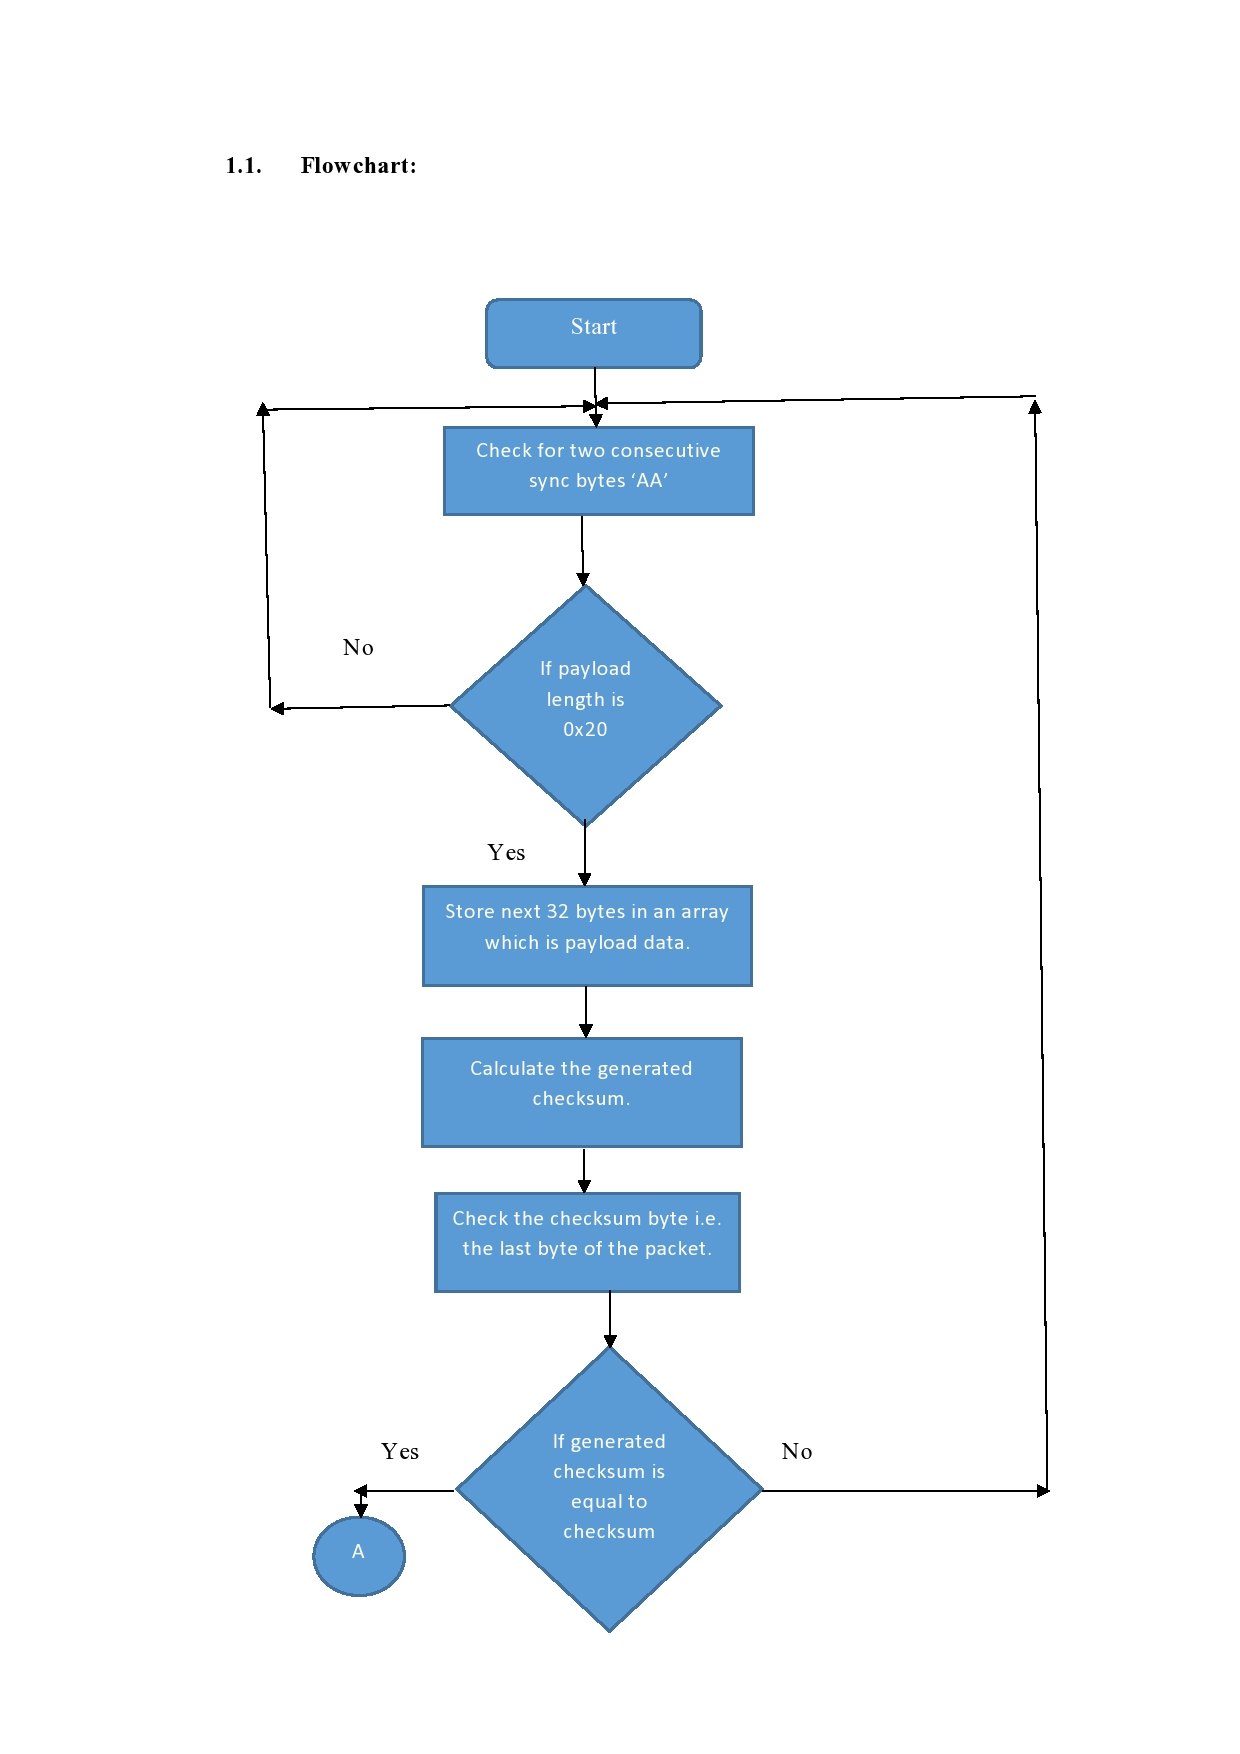
\includegraphics[width=19cm, height=24cm]{Att_Flow1}
\end{center}
\begin{center}
	\graphicspath{ {images/} }
	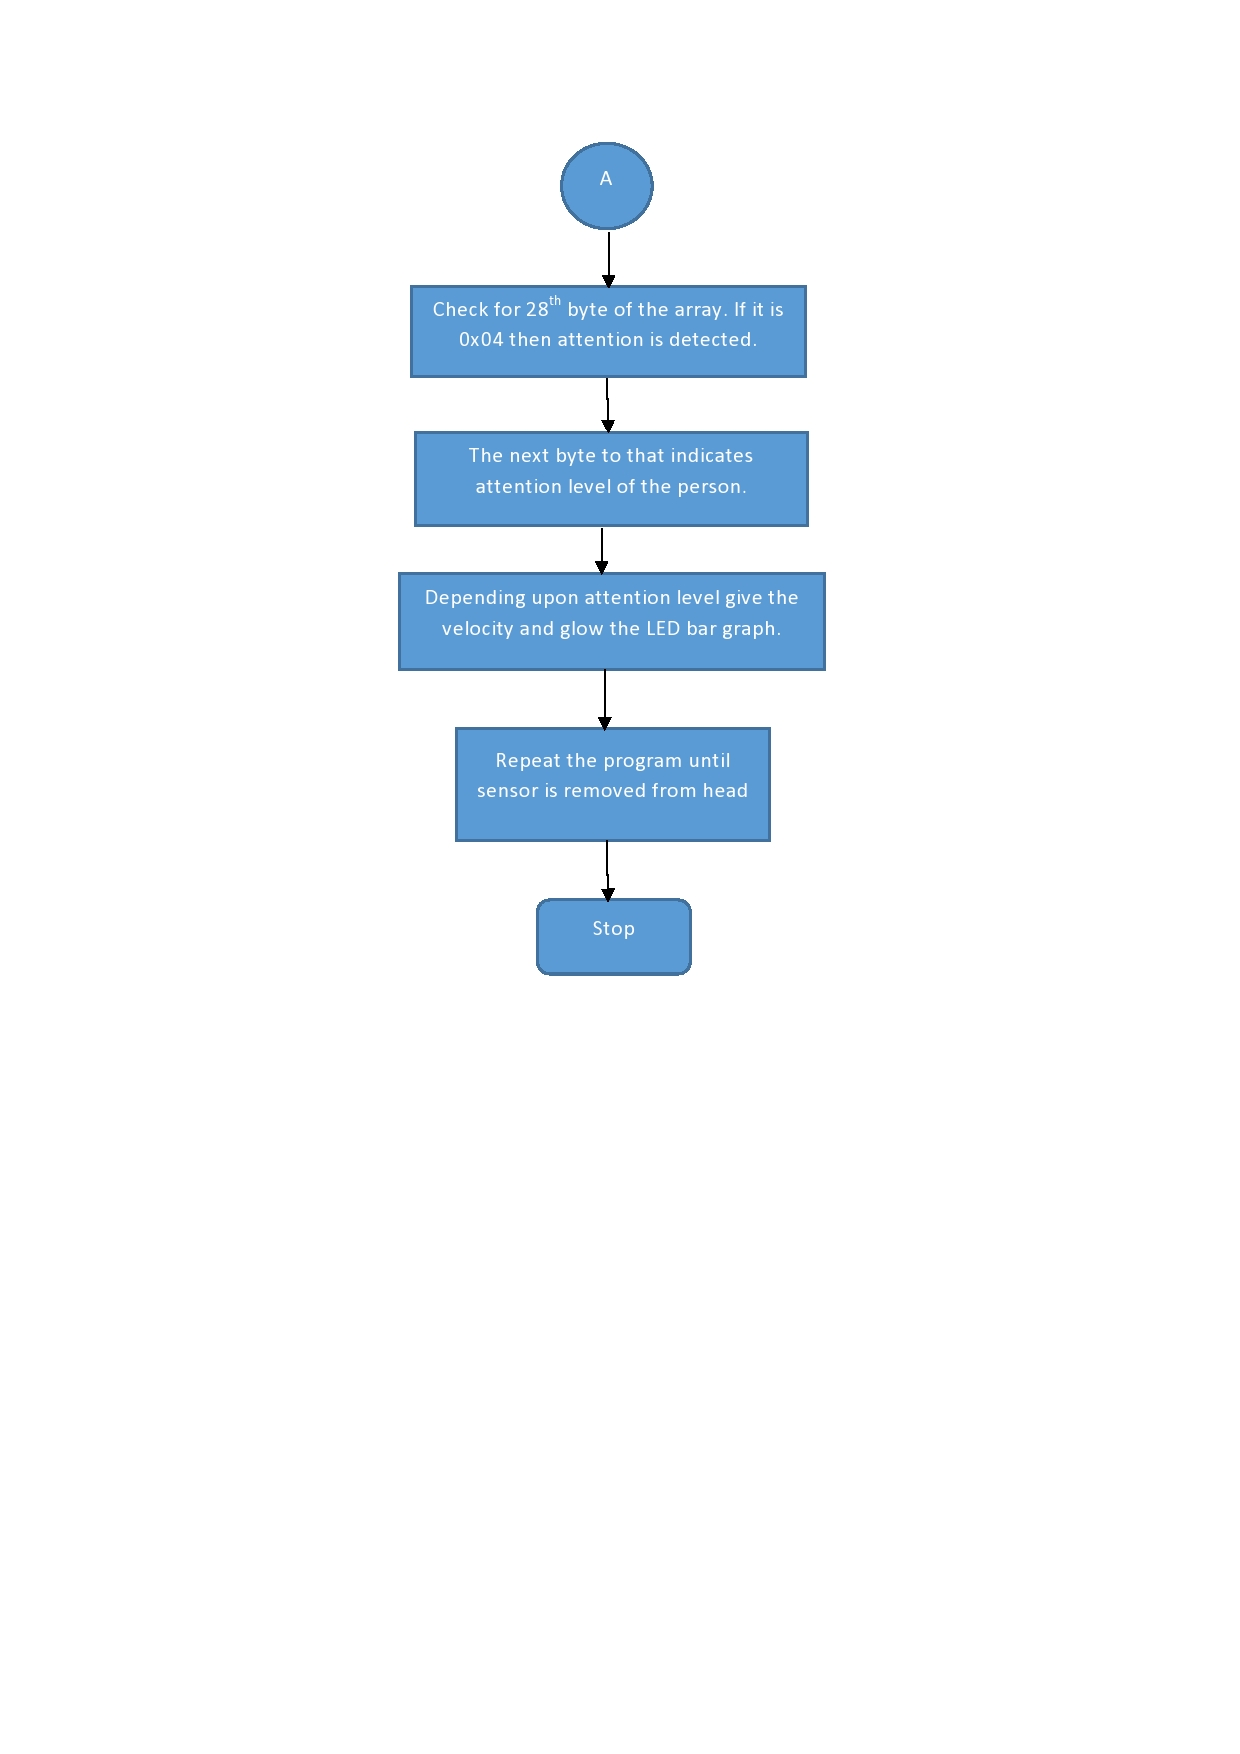
\includegraphics[width=19cm, height=24cm]{Att_Flow2}
\end{center}

\break


	\item \textbf{{\large Program to control Firebird V using Attention level and eye-blink.}}

\begin{enumerate}
	\item \textbf{Algorithm:}
\begin{enumerate}
\item Initialize all required ports.
\item Check for two consecutive SYNC bytes ‘AA’.
\item Check for third byte which is the payload length.
\item If payload length is 0x20, then store the next 32 bytes in an array. If payload length is 0x04 then move to step no. 11
\item Calculate the generated checksum.
\item If the last byte i.e. checksum byte of the data packet is equal to the generated checksum then check for 28th byte of the array.
\item If 28th byte is 0x04, then attention detected.
\item Then 29th byte indicates attention level of the person between 0-100.
\item Give velocity to the bot depending on the attention level.
\item Check for 1st byte of the array. If it is 0x02, then next byte to it should be 0x00, then eye-blink can be detected.
\item If payload length is 0x04, then store the next 4 bytes in an array.
\item Store the 1st and 2nd byte after 0x02 of the array in a variable and keep adding it for next 100 data packets.
\item  After taking average by 100, Eye-blink strength is between 110 and 350 and raw data values ranges above 350.
\item Now repeat from step 11 and 12 three times and check the eye-blink strength.
\item If eye- blink is given then its value will range between 110 and 350. 
\item Detection of such two eye-blinks will turn the bot left.
\item In order to stop the bot, remove the sensor from head. It will give values above 350.
\end{enumerate}

	\item \textbf{Flowchart:}
\end{enumerate}
\begin{center}
	\graphicspath{ {images/} }
	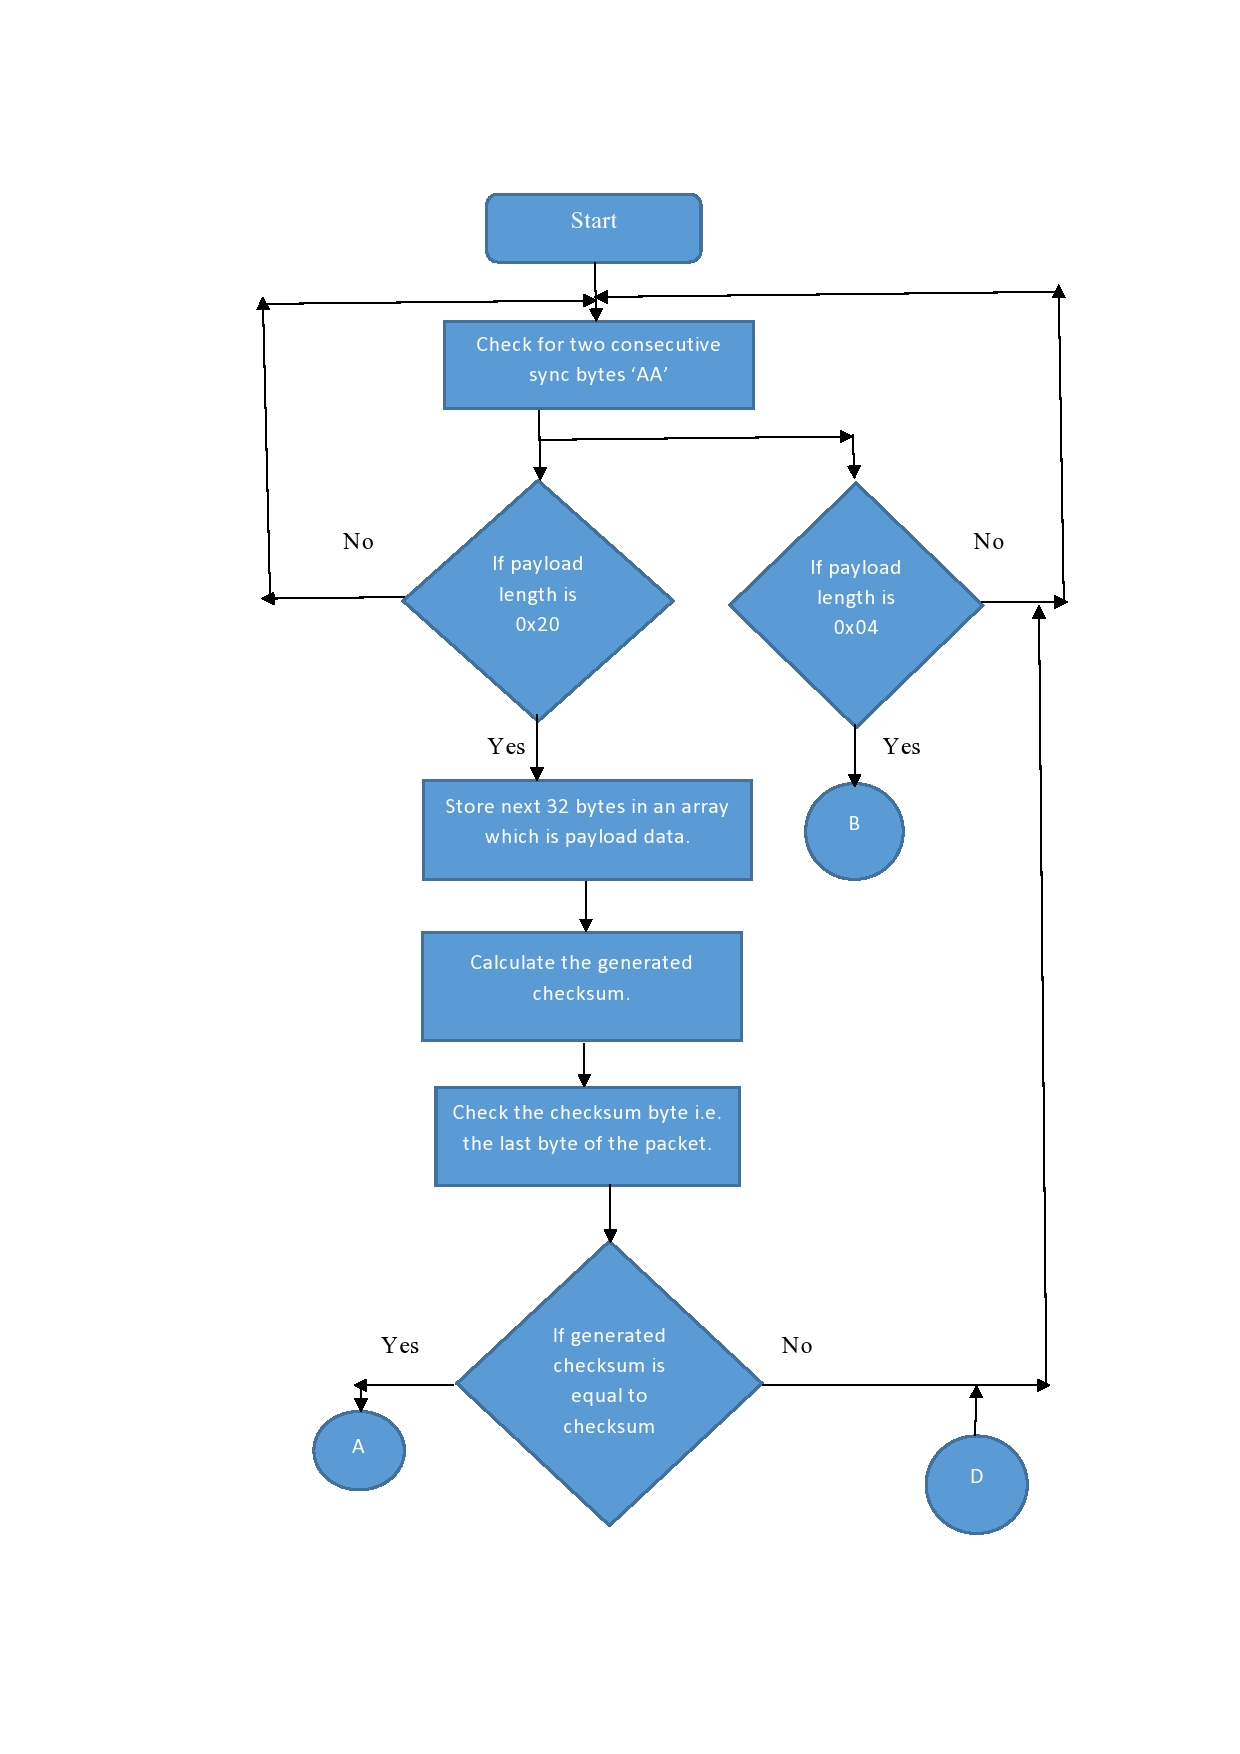
\includegraphics[width=18cm, height=23cm]{Flowchart1}
\end{center}
\begin{center}
	\graphicspath{ {images/} }
	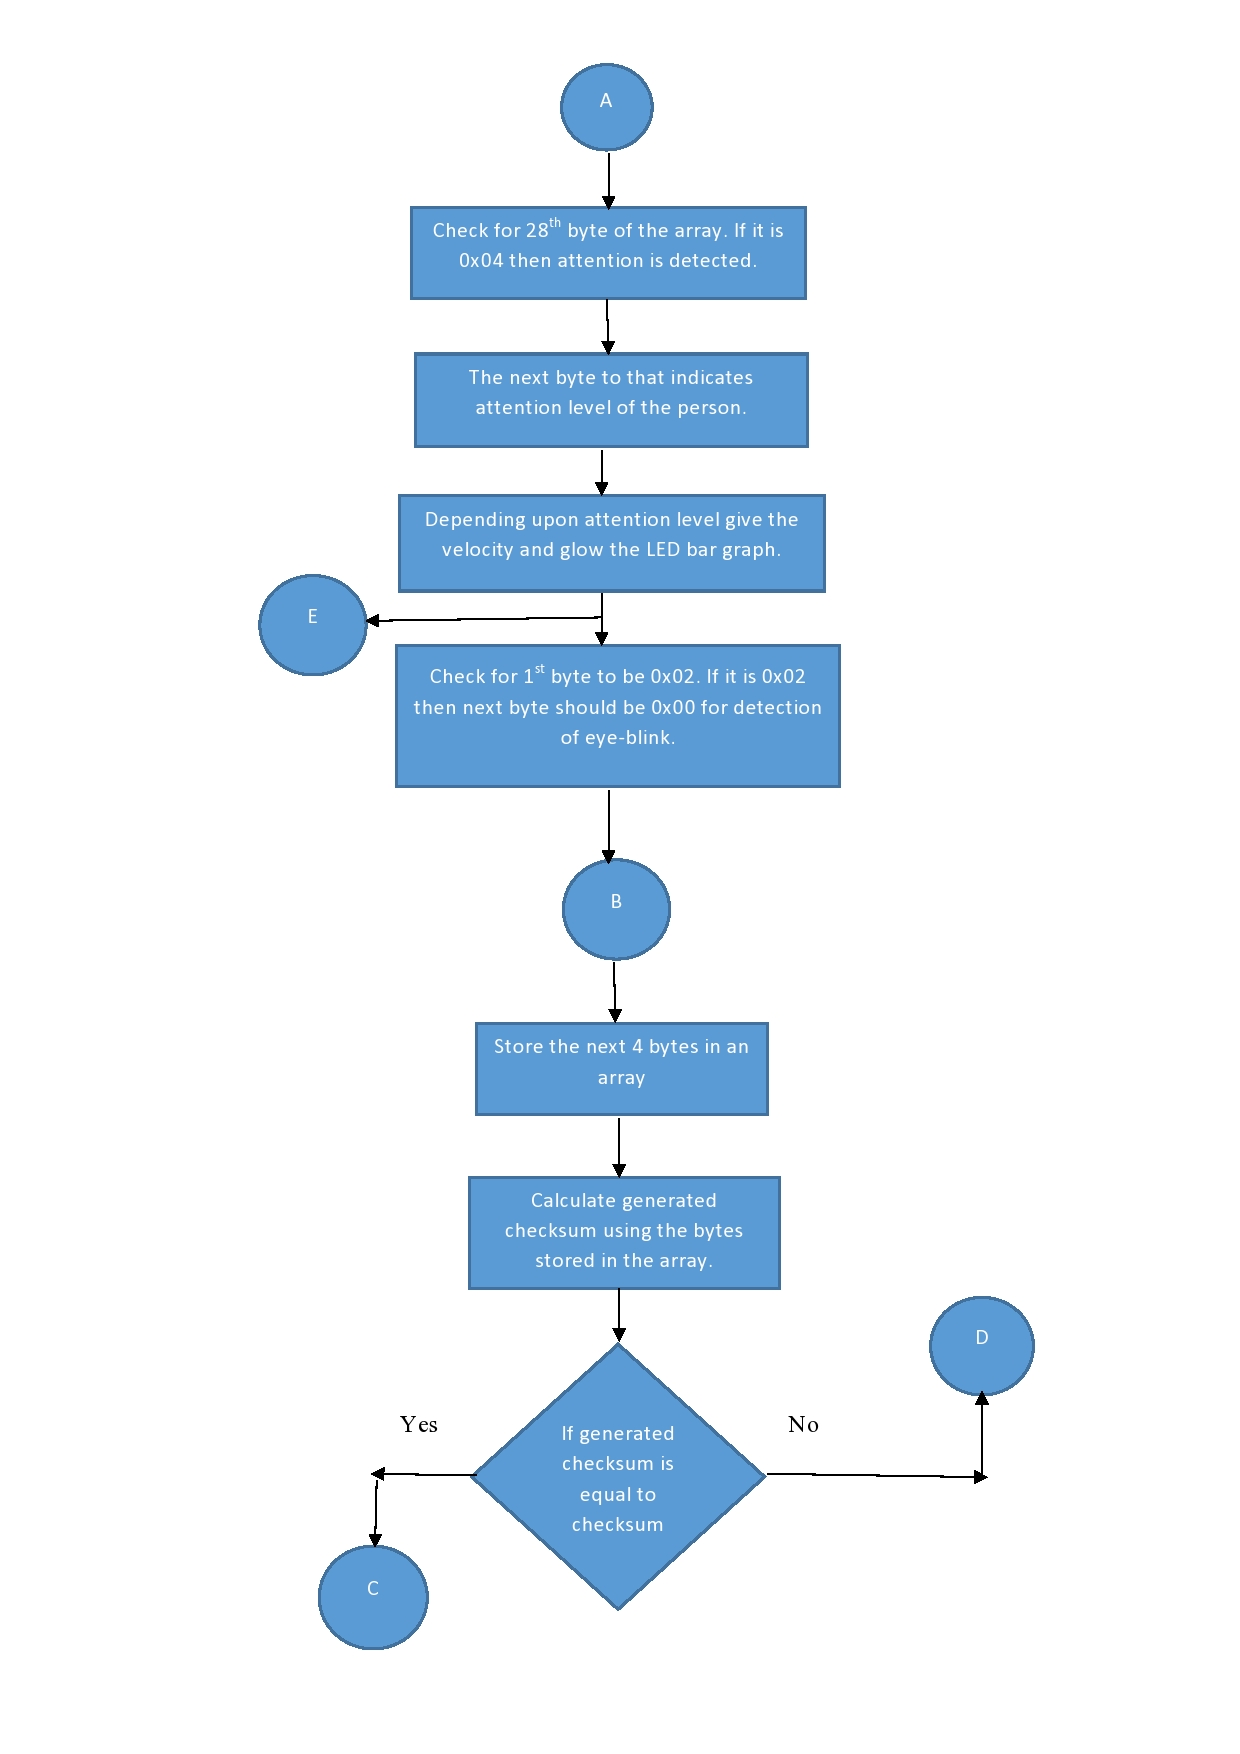
\includegraphics[width=19cm, height=24cm]{Flowchart2}
\end{center}
\begin{center}
	\graphicspath{ {images/} }
	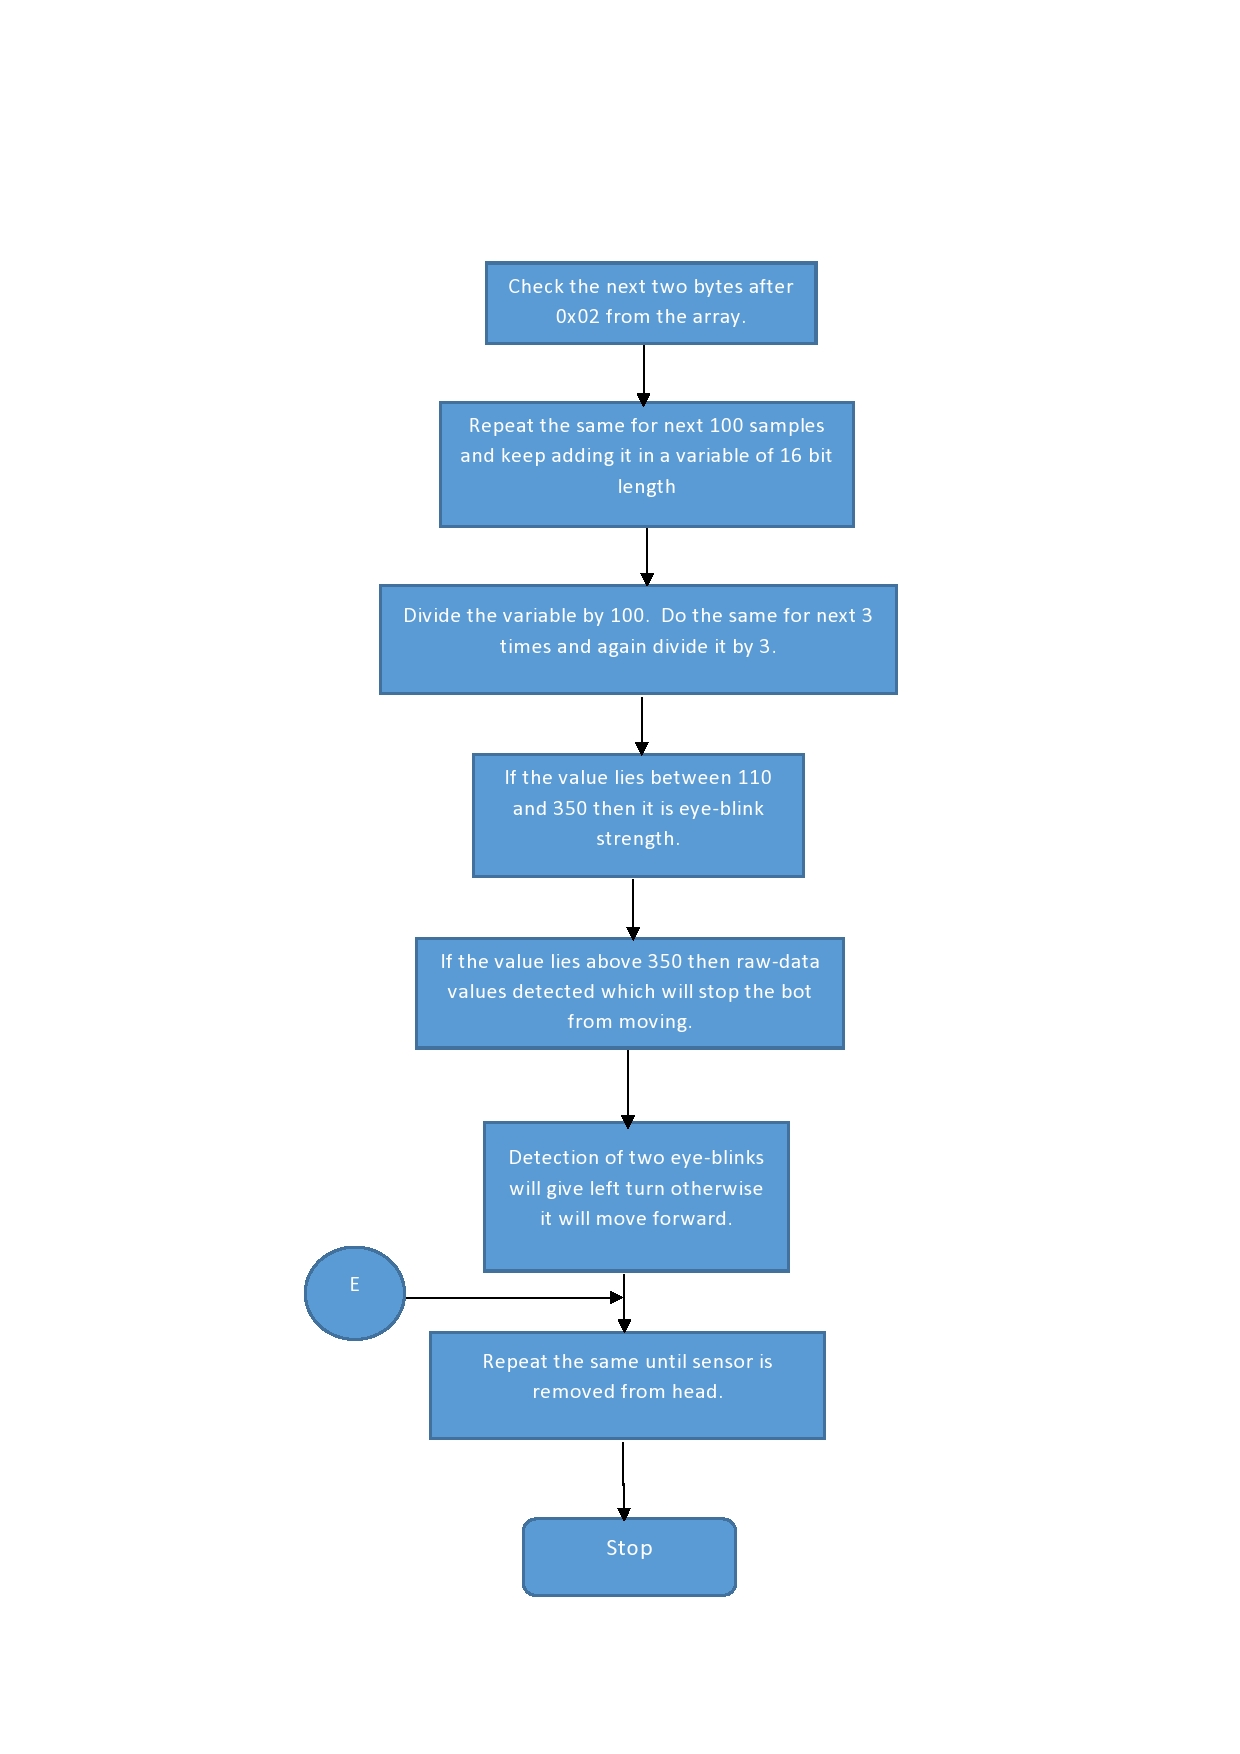
\includegraphics[width=19cm, height=24cm]{Flowchart3}
\end{center}
{\raggedright
In this way if you undeastand the concept of data pnckets aad analysed the data
vrlues properly it is ponsible to code for attentios level, eye-blink and also
for meditation level.
}
\end{enumerate}

\end{document}